\documentclass[prd,twocolumn,superscriptaddress,nofootinbib,showpacs,10pt]{revtex4-1}
\usepackage{amsmath,amssymb,graphicx,bm,float}
\usepackage{tikz}

\begin{document}

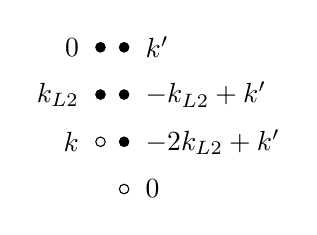
\begin{tikzpicture}[scale=.6,auto=left]

% Left column: filled and unfilled circles with left-aligned labels (top to bottom)
\draw[fill] (1,10) circle [radius=0.1cm];
\node [left] at (0.75,10) {$0$};

\draw[fill] (1,9) circle [radius=0.1cm];
\node [left] at (0.75,9) {$k_{L2}$};

\draw (1,8) circle [radius=0.1cm]; % unfilled
\node [left] at (0.75,8) {$k$};

% Right column: filled and unfilled circles with right-aligned labels (top to bottom)
\draw[fill] (1.5,10) circle [radius=0.1cm];
\node [right] at (1.75,10) {$k^\prime$};

\draw[fill] (1.5,9) circle [radius=0.1cm];
\node [right] at (1.75,9) {$-k_{L2}+k^\prime$};

\draw[fill] (1.5,8) circle [radius=0.1cm];
\node [right] at (1.75,8) {$-2k_{L2}+k^\prime$};

\draw (1.5,7) circle [radius=0.1cm]; % unfilled
\node [right] at (1.75,7) {$0$};

\end{tikzpicture}

\end{document}